% =============================================================================
% APPENDIX VI: FORMAL-MEQ - Multiple Equilibria & Strategic Navigation
% =============================================================================
% Category: FORMAL (Formalization)
% Language: English
% Version: 1.0 (January 2026)
% Dependencies: V (MEP), BB (EQUILIBRIA), HI (HIERARCHY), AW (BCJ)
%
% Purpose: Formalizes the identification, characterization, and navigation
% of multiple equilibria in behavioral intervention systems.
%
% Cross-Reference Map:
%   - Appendix CTW (MEP): Portfolio optimization foundation
%   - Appendix PAP (EQUILIBRIA): Tipping points and stability
%   - Appendix HIE (HIERARCHY): Decision level structure
%   - Appendix CAL1 (EIH): Intervention efficiency
%   - Appendix LET (LET): Level emergence
%   - Chapter 15: WEC Synthesis
%   - Chapter 17: Policy implications
% =============================================================================

\chapter{Multiple Equilibria \& Strategic Navigation (MEQ)}
\label{app:meq}

\begin{abstract}
The MEP optimization problem (Appendix CTW) is non-convex when complementarities
are positive ($\bar{\gamma} > 0$), implying the potential existence of multiple
local and global optima. This appendix formalizes the \textbf{Multiple Equilibria
Theorem (MEQ)}, which characterizes when multiple equilibria exist, how to identify
the current equilibrium state, how to map the complete equilibrium landscape, and
how to construct meta-strategic decision sets for practitioners. The framework
answers the fundamental question: \textit{Given where we are, where can we go,
how do we get there, and is it worth it?}
\end{abstract}

% -----------------------------------------------------------------------------
% APPENDIX SCOPE BOX
% -----------------------------------------------------------------------------

\begin{tcolorbox}[
    colback=orange!5!white,
    colframe=orange!75!black,
    title={\textbf{Appendix Scope: Ziel / In-Scope / Out-of-Scope / Constraints}},
    fonttitle=\bfseries
]

\textbf{Ziel (Objective):}
\begin{itemize}[nosep]
    \item Formalize and document the key concepts of Multiple Equilibria \& Strategic Navigation (MEQ)
\end{itemize}

\textbf{In-Scope:}
\begin{itemize}[nosep]
    \item Core theoretical foundations
    \item Mathematical formalizations where applicable
    \item Integration with EBF framework
\end{itemize}

\textbf{Out-of-Scope (delegiert an andere Appendices):}
\begin{itemize}[nosep]
    \item Detailed empirical validation $\rightarrow$ METHOD appendices
    \item Domain-specific applications $\rightarrow$ DOMAIN appendices
    \item Complete literature review $\rightarrow$ LIT appendices
\end{itemize}

\textbf{Constraints (Anwendungsgrenzen):}
\begin{itemize}[nosep]
    \item Framework requires calibration to specific contexts
    \item Parameters may vary across domains
    \item Validity bounded by underlying assumptions
\end{itemize}

\textbf{Lieferobjekte (Deliverables):}
\begin{itemize}[nosep]
    \item Theoretical framework with formal definitions
    \item Integration points with other appendices
    \item Practical guidelines for application
\end{itemize}

\end{tcolorbox}



\begin{tcolorbox}[colback=blue!5!white, colframe=blue!75!black,
    title=Quick Reference: Multiple Equilibria \& Strategic Navigation (MEQ)]

\textbf{Appendix:} MEQ (FORMAL)

\textbf{Core Concepts:}
\begin{itemize}[nosep]
\item Complementarity ($\gamma > 0$): Components interact synergistically
\item Context ($\Psi$): Situational factors that influence behavior
\item Utility dimensions: FEPSDE (Financial, Emotional, Physical, Social, Development, Experiential)
\end{itemize}

\textbf{Key Formulas:}
\begin{equation}
U = \sum_d \omega_d \cdot u_d + \gamma \cdot f(\text{interactions})
\end{equation}

\textbf{Cross-References:} Appendix B (CORE-HOW), V (CORE-WHEN), G (Glossary)
\end{tcolorbox}



%%%%%%%%%%%%%%%%%%%%%%%%%%%%%%%%%%%%%%%%%%%%%%%%%%%%%%%%%%%%%%%%%%%%%%%%%%%%%%%
\section{The Strategic Navigation Problem}
\label{sec:meq-problem}
%%%%%%%%%%%%%%%%%%%%%%%%%%%%%%%%%%%%%%%%%%%%%%%%%%%%%%%%%%%%%%%%%%%%%%%%%%%%%%%

\begin{tcolorbox}[colback=blue!5!white, colframe=blue!75!black,
    title=The Five Questions of Strategic Navigation]

Every behavioral intervention decision ultimately requires answering:

\begin{enumerate}
    \item \textbf{DIAGNOSE:} In which equilibrium are we currently?
    \item \textbf{MAP:} What other equilibria exist in the landscape?
    \item \textbf{PATH:} What intervention mix reaches each equilibrium?
    \item \textbf{FEASIBLE:} Is the transition realistic given constraints?
    \item \textbf{DECIDE:} What meta-strategic alternatives should we present?
\end{enumerate}

\textbf{Key Insight:} The MEP (Appendix CTW) finds the cost-minimizing portfolio
for a \textit{given} target. MEQ addresses the prior question: \textit{Which
targets should we even consider?}

\end{tcolorbox}

\subsection{Formal Problem Statement}

Let the behavioral system be characterized by:
\begin{itemize}[nosep]
    \item Current state: $S_0 = (WEC_0, \varphi_0, L_0)$ where $WEC_0$ is current
          willingness-to-change, $\varphi_0$ is BCJ phase, $L_0$ is primary decision level
    \item Intervention space: $\mathcal{W} = \{w \in \mathbb{R}^n_+ : \sum_i w_i \leq B\}$
    \item Outcome function: $WEC(w) = E'w + w'\Gamma^{eff}w$
    \item Cost function: $C(w) = c'w$
    \item Constraint set: $\mathcal{C} = \{w : g_j(w) \leq 0, j = 1,...,m\}$
\end{itemize}

The \textbf{equilibrium landscape} is defined as:
\begin{equation}
\boxed{
\mathcal{E} = \left\{ S^* : S^* = \lim_{t \to \infty} S(t; w^*) \text{ for some } w^* \in \mathcal{W} \cap \mathcal{C} \right\}
}
\end{equation}

%%%%%%%%%%%%%%%%%%%%%%%%%%%%%%%%%%%%%%%%%%%%%%%%%%%%%%%%%%%%%%%%%%%%%%%%%%%%%%%
\section{The Multiple Equilibria Theorem}
\label{sec:meq-theorem}
%%%%%%%%%%%%%%%%%%%%%%%%%%%%%%%%%%%%%%%%%%%%%%%%%%%%%%%%%%%%%%%%%%%%%%%%%%%%%%%

\begin{tcolorbox}[colback=red!5!white, colframe=red!75!black,
    title=Theorem MEQ-1: Existence of Multiple Equilibria]

\textbf{Multiple Equilibria Theorem (MEQ-1):}

Let $\Gamma^{eff}$ be the effective complementarity matrix with eigenvalues
$\{\lambda_1, ..., \lambda_n\}$. Define:
\begin{itemize}[nosep]
    \item $n_+ = |\{i : \lambda_i > 0\}|$ (number of positive eigenvalues)
    \item $n_- = |\{i : \lambda_i < 0\}|$ (number of negative eigenvalues)
    \item $n_0 = |\{i : \lambda_i = 0\}|$ (number of zero eigenvalues)
\end{itemize}

Then:

\begin{enumerate}
    \item \textbf{Unique Equilibrium:} If $n_+ = 0$ (all eigenvalues $\leq 0$),
          then $|\mathcal{E}| = 1$ (unique global optimum)

    \item \textbf{Multiple Equilibria:} If $n_+ \geq 1$ and $n_- \geq 1$, then
          $|\mathcal{E}| \geq 2$ (at least two distinct equilibria)

    \item \textbf{Upper Bound:} $|\mathcal{E}| \leq 2^{n_+}$ (exponential in
          positive eigenvalue count)
\end{enumerate}

\end{tcolorbox}

\subsection{Proof of MEQ-1}

\begin{proof}
The MEP objective function is:
\begin{equation}
f(w) = c'w - \mu(E'w + w'\Gamma^{eff}w - \Delta WEC^*)
\end{equation}

The Hessian is:
\begin{equation}
H = -2\mu \Gamma^{eff}
\end{equation}

\textbf{Part 1 (Unique):} If all eigenvalues of $\Gamma^{eff}$ are $\leq 0$, then
$H$ is positive semi-definite (for $\mu > 0$), making $f$ concave. Maximizing a
concave function over a convex set yields a unique global maximum.

\textbf{Part 2 (Multiple):} If $\Gamma^{eff}$ has both positive and negative
eigenvalues, $H$ is indefinite. The objective has saddle points, and the constraint
boundary $WEC(w) = \Delta WEC^*$ is non-convex. By Morse theory, a non-degenerate
critical point with $k$ negative eigenvalues contributes to the topology, implying
multiple local optima.

\textbf{Part 3 (Bound):} Each positive eigenvalue creates a direction where the
constraint surface curves ``outward,'' potentially creating a separate basin of
attraction. The maximum number of such basins is $2^{n_+}$.
\end{proof}

\subsection{Equilibrium Classification}

\begin{definition}[Equilibrium Types]
We classify equilibria by their structural properties:

\begin{table}[H]
\centering
\caption{Equilibrium Type Classification}
\label{tab:meq-types}
\renewcommand{\arraystretch}{1.4}
\begin{tabular}{@{}llll@{}}
\toprule
\textbf{Type} & \textbf{Symbol} & \textbf{Characterization} & \textbf{Portfolio Structure} \\
\midrule
Low-Intensity & $E_{LI}$ & Many weak interventions & $w_i \approx \bar{w}$ for all $i$ \\
High-Intensity & $E_{HI}$ & Few strong interventions & $w_i^* \gg 0$ for $|\{i\}| \leq 3$ \\
Synergy & $E_{SY}$ & Complementary pairs/triples & $w_i, w_j > 0$ where $\gamma_{ij} \gg 0$ \\
Substitution & $E_{SU}$ & Diversified, low correlation & $w_i > 0$ where $\gamma_{ij} < 0$ \\
Hybrid & $E_{HY}$ & Mixed structure & Combination of above \\
\bottomrule
\end{tabular}
\end{table}
\end{definition}

%%%%%%%%%%%%%%%%%%%%%%%%%%%%%%%%%%%%%%%%%%%%%%%%%%%%%%%%%%%%%%%%%%%%%%%%%%%%%%%
\section{Phase 1: Equilibrium Diagnosis}
\label{sec:meq-diagnosis}
%%%%%%%%%%%%%%%%%%%%%%%%%%%%%%%%%%%%%%%%%%%%%%%%%%%%%%%%%%%%%%%%%%%%%%%%%%%%%%%

\begin{tcolorbox}[colback=green!5!white, colframe=green!75!black,
    title=Question 1: Where Are We Now?]

\textbf{Diagnostic Protocol:}

Given observable data $(WEC_{obs}, \varphi_{obs}, w_{current})$, identify the
current equilibrium $E_0 \in \mathcal{E}$.

\end{tcolorbox}

\subsection{The Diagnostic Function}

\begin{definition}[Equilibrium Signature]
Each equilibrium $E^* \in \mathcal{E}$ has a unique \textbf{signature}:
\begin{equation}
\sigma(E^*) = \left( WEC^*, \varphi^*, L^*, \text{Type}^*, \text{Basin}^* \right)
\end{equation}
where:
\begin{itemize}[nosep]
    \item $WEC^*$ = equilibrium willingness-to-change level
    \item $\varphi^*$ = stable BCJ phase
    \item $L^*$ = primary decision level
    \item $\text{Type}^* \in \{E_{LI}, E_{HI}, E_{SY}, E_{SU}, E_{HY}\}$
    \item $\text{Basin}^*$ = basin of attraction (set of initial conditions converging to $E^*$)
\end{itemize}
\end{definition}

\subsection{Diagnostic Algorithm}

\begin{algorithm}[H]
\caption{Equilibrium Diagnosis (DIAG)}
\label{alg:diagnosis}
\begin{algorithmic}[1]
\Require Current state $(WEC_{obs}, \varphi_{obs}, w_{current})$
\Ensure Current equilibrium identification $E_0$

\State \textbf{Step 1: Stability Test}
\State Compute $\nabla WEC(w_{current})$ and $H(w_{current})$
\If{$\|\nabla WEC\| < \epsilon$ and $H$ is locally stable}
    \State $E_0 \gets$ current state is at equilibrium
\Else
    \State $E_0 \gets$ system is in transition
\EndIf

\State \textbf{Step 2: Type Classification}
\State Compute Herfindahl index: $HHI = \sum_i (w_i / \sum_j w_j)^2$
\State Compute synergy ratio: $SR = \sum_{i<j} \gamma_{ij} w_i w_j / (w'\Gamma w)$
\If{$HHI > 0.5$}
    \State Type $\gets E_{HI}$
\ElsIf{$SR > 0.7$}
    \State Type $\gets E_{SY}$
\ElsIf{$SR < 0.3$ and $\bar{\gamma} < 0$}
    \State Type $\gets E_{SU}$
\Else
    \State Type $\gets E_{HY}$
\EndIf

\State \textbf{Step 3: Signature Construction}
\State $\sigma(E_0) \gets (WEC_{obs}, \varphi_{obs}, L_{obs}, \text{Type}, \text{Basin})$

\Return $E_0, \sigma(E_0)$
\end{algorithmic}
\end{algorithm}

%%%%%%%%%%%%%%%%%%%%%%%%%%%%%%%%%%%%%%%%%%%%%%%%%%%%%%%%%%%%%%%%%%%%%%%%%%%%%%%
\section{Phase 2: Equilibrium Landscape Mapping}
\label{sec:meq-landscape}
%%%%%%%%%%%%%%%%%%%%%%%%%%%%%%%%%%%%%%%%%%%%%%%%%%%%%%%%%%%%%%%%%%%%%%%%%%%%%%%

\begin{tcolorbox}[colback=green!5!white, colframe=green!75!black,
    title=Question 2: What Other Equilibria Exist?]

\textbf{Mapping Protocol:}

Enumerate all equilibria $\mathcal{E} = \{E_1, E_2, ..., E_K\}$ reachable from
the current state under budget constraint $B$.

\end{tcolorbox}

\subsection{The Landscape Theorem}

\begin{theorem}[Equilibrium Landscape Structure (MEQ-2)]
\label{thm:meq-landscape}

For intervention dimension $n$ and complementarity matrix $\Gamma^{eff}$ with
signature $(n_+, n_-, n_0)$, the equilibrium landscape has structure:

\begin{enumerate}
    \item \textbf{Layered Structure:} Equilibria organize into ``shells'' by WEC level:
    \begin{equation}
    \mathcal{E} = \bigcup_{k=1}^{K} \mathcal{E}_k \quad \text{where } \mathcal{E}_k = \{E : WEC(E) \in [W_k, W_{k+1})\}
    \end{equation}

    \item \textbf{Connectivity:} Two equilibria $E_i, E_j$ are connected if there
    exists a continuous path $w(t)$ with $w(0) \in \text{Basin}(E_i)$ and
    $w(1) \in \text{Basin}(E_j)$.

    \item \textbf{Hierarchy:} There exists a partial ordering $\preceq$ on $\mathcal{E}$
    such that $E_i \preceq E_j$ implies $WEC(E_i) \leq WEC(E_j)$ and transition
    $E_i \to E_j$ requires positive net investment.
\end{enumerate}
\end{theorem}

\subsection{Landscape Mapping Algorithm}

\begin{algorithm}[H]
\caption{Equilibrium Landscape Mapping (MAP)}
\label{alg:landscape}
\begin{algorithmic}[1]
\Require Complementarity matrix $\Gamma^{eff}$, cost vector $c$, budget $B$
\Ensure Equilibrium set $\mathcal{E}$ with signatures

\State \textbf{Step 1: Eigendecomposition}
\State $\Gamma^{eff} = V \Lambda V'$ where $\Lambda = \text{diag}(\lambda_1, ..., \lambda_n)$
\State $n_+ \gets |\{i : \lambda_i > 0\}|$

\State \textbf{Step 2: Critical Point Enumeration}
\For{each subset $S \subseteq \{1, ..., n\}$ with $|S| \leq n_+$}
    \State Solve KKT conditions for $w$ active on $S$
    \State If solution exists and $C(w) \leq B$, add to candidate set
\EndFor

\State \textbf{Step 3: Stability Classification}
\For{each candidate $w^*$}
    \State Compute bordered Hessian $\bar{H}$
    \If{$\bar{H}$ satisfies second-order conditions}
        \State Add $E^* = (w^*, WEC(w^*), \text{Type})$ to $\mathcal{E}$
    \EndIf
\EndFor

\State \textbf{Step 4: Basin Computation}
\For{each $E^* \in \mathcal{E}$}
    \State Compute local basin via gradient flow analysis
    \State $\text{Basin}(E^*) \gets \{w_0 : \lim_{t \to \infty} w(t; w_0) = w^*\}$
\EndFor

\Return $\mathcal{E}$ with complete signatures
\end{algorithmic}
\end{algorithm}

\subsection{Visualization: The Equilibrium Map}

\begin{figure}[H]
\centering
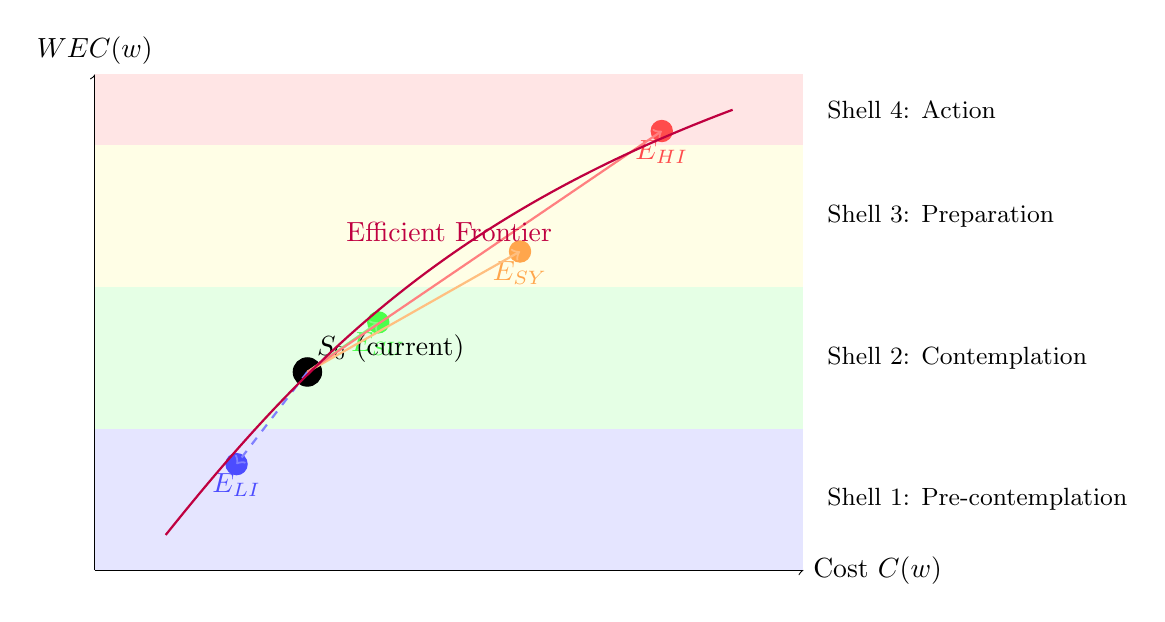
\begin{tikzpicture}[scale=0.9]
% Axes
\draw[->] (0,0) -- (10,0) node[right] {Cost $C(w)$};
\draw[->] (0,0) -- (0,7) node[above] {$WEC(w)$};

% Equilibrium shells
\fill[blue!10] (0,0) rectangle (10,2);
\fill[green!10] (0,2) rectangle (10,4);
\fill[yellow!10] (0,4) rectangle (10,6);
\fill[red!10] (0,6) rectangle (10,7);

% Shell labels
\node[right] at (10.2,1) {\small Shell 1: Pre-contemplation};
\node[right] at (10.2,3) {\small Shell 2: Contemplation};
\node[right] at (10.2,5) {\small Shell 3: Preparation};
\node[right] at (10.2,6.5) {\small Shell 4: Action};

% Equilibria
\filldraw[blue!70] (2,1.5) circle (0.15) node[below] {$E_{LI}$};
\filldraw[green!70] (4,3.5) circle (0.15) node[below] {$E_{SU}$};
\filldraw[orange!70] (6,4.5) circle (0.15) node[below] {$E_{SY}$};
\filldraw[red!70] (8,6.2) circle (0.15) node[below] {$E_{HI}$};

% Current state
\filldraw[black] (3,2.8) circle (0.2) node[above right] {$S_0$ (current)};

% Transition paths
\draw[->, thick, dashed, blue!50] (3,2.8) -- (2,1.5);
\draw[->, thick, green!50] (3,2.8) -- (4,3.5);
\draw[->, thick, orange!50] (3,2.8) -- (6,4.5);
\draw[->, thick, red!50] (3,2.8) -- (8,6.2);

% Efficient frontier
\draw[thick, purple] (1,0.5) .. controls (3,3) and (5,5) .. (9,6.5);
\node[purple, above] at (5,4.5) {Efficient Frontier};

\end{tikzpicture}
\caption{Equilibrium Landscape Map showing four equilibria across BCJ shells,
with current state $S_0$ and possible transition paths.}
\label{fig:meq-landscape}
\end{figure}

%%%%%%%%%%%%%%%%%%%%%%%%%%%%%%%%%%%%%%%%%%%%%%%%%%%%%%%%%%%%%%%%%%%%%%%%%%%%%%%
\section{Phase 3: Transition Path Analysis}
\label{sec:meq-transition}
%%%%%%%%%%%%%%%%%%%%%%%%%%%%%%%%%%%%%%%%%%%%%%%%%%%%%%%%%%%%%%%%%%%%%%%%%%%%%%%

\begin{tcolorbox}[colback=green!5!white, colframe=green!75!black,
    title=Question 3: How Do We Get There?]

\textbf{Path Protocol:}

For each target equilibrium $E^* \in \mathcal{E}$, compute the optimal transition
path and required intervention portfolio.

\end{tcolorbox}

\subsection{Transition Path Theorem}

\begin{theorem}[Optimal Transition Path (MEQ-3)]
\label{thm:meq-transition}

Let $E_0$ be the current equilibrium and $E^*$ be the target. The optimal
transition path $w^*(t)$ solves:

\begin{equation}
\boxed{
\min_{w(t)} \int_0^T C(w(t)) dt \quad \text{s.t.} \quad
\begin{cases}
\dot{S}(t) = f(S(t), w(t)) \\
S(0) = S_0 \\
S(T) \in \text{Basin}(E^*)
\end{cases}
}
\end{equation}

The solution satisfies the \textbf{Transition Euler Equation}:
\begin{equation}
c_i = \mu(t) \cdot \frac{\partial f}{\partial w_i} + \dot{\mu}(t) \cdot \frac{\partial f}{\partial S}
\end{equation}
where $\mu(t)$ is the costate variable (shadow value of state advancement).
\end{theorem}

\subsection{Transition Taxonomy}

\begin{definition}[Transition Types]
Transitions between equilibria are classified by their characteristics:

\begin{table}[H]
\centering
\caption{Transition Type Classification}
\label{tab:meq-transitions}
\renewcommand{\arraystretch}{1.4}
\begin{tabular}{@{}lllll@{}}
\toprule
\textbf{Type} & \textbf{Symbol} & \textbf{Mechanism} & \textbf{Cost Profile} & \textbf{Risk} \\
\midrule
Gradual & $T_G$ & Continuous adjustment & Linear & Low \\
Threshold & $T_T$ & Discrete jump at tipping point & Step function & Medium \\
Cascade & $T_C$ & Self-reinforcing sequence & Front-loaded & Medium \\
Transformational & $T_X$ & Regime change & High initial, declining & High \\
Reversible & $T_R$ & Temporary shift & Symmetric & Low \\
\bottomrule
\end{tabular}
\end{table}
\end{definition}

\subsection{The Transition Matrix}

\begin{definition}[Transition Cost Matrix]
For equilibrium set $\mathcal{E} = \{E_1, ..., E_K\}$, define the
\textbf{Transition Cost Matrix} $\mathbf{T}$:
\begin{equation}
T_{ij} = \min_{w} \int_0^{T_{ij}} C(w(t)) dt \quad \text{s.t. } E_i \to E_j
\end{equation}
where $T_{ij}$ is the minimum transition time from $E_i$ to $E_j$.

Properties:
\begin{itemize}[nosep]
    \item $T_{ii} = 0$ (no cost to stay)
    \item $T_{ij} \neq T_{ji}$ in general (asymmetric transitions)
    \item $T_{ij} = \infty$ if transition is infeasible
\end{itemize}
\end{definition}

\subsection{Intervention Portfolio for Each Transition}

For each feasible transition $E_i \to E_j$, the required intervention portfolio is:

\begin{equation}
w^*_{i \to j} = \arg\min_{w} C(w) \quad \text{s.t.} \quad
\begin{cases}
WEC(w) \geq WEC(E_j) - WEC(E_i) \\
w \in \text{Basin}(E_j) \\
g_k(w) \leq 0 \quad \forall k
\end{cases}
\end{equation}

%%%%%%%%%%%%%%%%%%%%%%%%%%%%%%%%%%%%%%%%%%%%%%%%%%%%%%%%%%%%%%%%%%%%%%%%%%%%%%%
\section{Phase 4: Feasibility Assessment}
\label{sec:meq-feasibility}
%%%%%%%%%%%%%%%%%%%%%%%%%%%%%%%%%%%%%%%%%%%%%%%%%%%%%%%%%%%%%%%%%%%%%%%%%%%%%%%

\begin{tcolorbox}[colback=green!5!white, colframe=green!75!black,
    title=Question 4: Is It Realistic?]

\textbf{Feasibility Protocol:}

For each potential transition, assess whether it is realistically achievable
given organizational, temporal, and resource constraints.

\end{tcolorbox}

\subsection{The Feasibility Function}

\begin{definition}[Multi-Dimensional Feasibility]
The feasibility of transition $E_i \to E_j$ is assessed across five dimensions:

\begin{equation}
\mathcal{F}_{i \to j} = \prod_{d=1}^{5} F_d(E_i, E_j)
\end{equation}

where:
\begin{align}
F_1 &= \text{Budget Feasibility} = \mathbb{1}[T_{ij} \leq B] \\
F_2 &= \text{Time Feasibility} = \mathbb{1}[T_{ij}^{time} \leq T_{max}] \\
F_3 &= \text{Capability Feasibility} = \prod_k \mathbb{1}[w^*_k \leq \text{Cap}_k] \\
F_4 &= \text{Political Feasibility} = P(\text{approval} | w^*_{i \to j}) \\
F_5 &= \text{Risk Feasibility} = \mathbb{1}[\text{VaR}(w^*) \leq \text{Risk}_{max}]
\end{align}
\end{definition}

\subsection{Feasibility Assessment Algorithm}

\begin{algorithm}[H]
\caption{Feasibility Assessment (FEAS)}
\label{alg:feasibility}
\begin{algorithmic}[1]
\Require Transition $E_i \to E_j$, constraints $(B, T_{max}, \text{Cap}, P_{min}, \text{Risk}_{max})$
\Ensure Feasibility score $\mathcal{F}_{i \to j}$ and binding constraints

\State \textbf{Step 1: Budget Check}
\State $F_1 \gets \mathbb{1}[T_{ij} \leq B]$
\If{$F_1 = 0$}
    \State $\text{Binding} \gets \text{Binding} \cup \{\text{Budget}\}$
\EndIf

\State \textbf{Step 2: Time Check}
\State Compute minimum transition time $T_{ij}^{time}$
\State $F_2 \gets \mathbb{1}[T_{ij}^{time} \leq T_{max}]$

\State \textbf{Step 3: Capability Check}
\For{each intervention $k$ with $w^*_k > 0$}
    \If{$w^*_k > \text{Cap}_k$}
        \State $F_3 \gets 0$; $\text{Binding} \gets \text{Binding} \cup \{\text{Capability}_k\}$
    \EndIf
\EndFor

\State \textbf{Step 4: Political Check}
\State Estimate approval probability $P(\text{approval} | w^*)$
\State $F_4 \gets P$ (continuous score in $[0,1]$)

\State \textbf{Step 5: Risk Check}
\State Compute Value-at-Risk: $\text{VaR}(w^*) = F^{-1}_{WEC}(0.05)$
\State $F_5 \gets \mathbb{1}[\text{VaR}(w^*) \geq \text{WEC}_{min}]$

\State \textbf{Step 6: Aggregate}
\State $\mathcal{F}_{i \to j} \gets F_1 \cdot F_2 \cdot F_3 \cdot F_4 \cdot F_5$

\Return $\mathcal{F}_{i \to j}$, Binding constraints
\end{algorithmic}
\end{algorithm}

\subsection{The Feasibility Matrix}

\begin{definition}[Feasibility Matrix]
The \textbf{Feasibility Matrix} $\mathbf{F}$ captures pairwise transition feasibility:
\begin{equation}
F_{ij} = \mathcal{F}_{i \to j} \in [0, 1]
\end{equation}

The \textbf{Feasible Transition Set} from current equilibrium $E_0$ is:
\begin{equation}
\mathcal{E}^{feasible}(E_0) = \{E_j \in \mathcal{E} : F_{0j} > F_{min}\}
\end{equation}
\end{definition}

%%%%%%%%%%%%%%%%%%%%%%%%%%%%%%%%%%%%%%%%%%%%%%%%%%%%%%%%%%%%%%%%%%%%%%%%%%%%%%%
\section{Phase 5: Meta-Strategic Decision Set}
\label{sec:meq-decision}
%%%%%%%%%%%%%%%%%%%%%%%%%%%%%%%%%%%%%%%%%%%%%%%%%%%%%%%%%%%%%%%%%%%%%%%%%%%%%%%

\begin{tcolorbox}[colback=green!5!white, colframe=green!75!black,
    title=Question 5: What Are the Strategic Alternatives?]

\textbf{Decision Protocol:}

Construct the meta-strategic decision set $\mathcal{D}$ presenting all viable
strategic alternatives to the decision-maker.

\end{tcolorbox}

\subsection{The Meta-Strategic Decision Set}

\begin{definition}[Strategic Alternative]
A \textbf{Strategic Alternative} $A_k$ is a tuple:
\begin{equation}
A_k = \left( E^{target}_k, w^*_k, T_k, C_k, \mathcal{F}_k, \text{ROI}_k, \text{Risk}_k \right)
\end{equation}
where:
\begin{itemize}[nosep]
    \item $E^{target}_k$ = target equilibrium
    \item $w^*_k$ = optimal intervention portfolio
    \item $T_k$ = transition time
    \item $C_k$ = total cost
    \item $\mathcal{F}_k$ = feasibility score
    \item $\text{ROI}_k = \Delta WEC_k / C_k$ = return on investment
    \item $\text{Risk}_k$ = transition risk measure
\end{itemize}
\end{definition}

\begin{definition}[Meta-Strategic Decision Set]
The \textbf{Meta-Strategic Decision Set} $\mathcal{D}$ is the set of all
Pareto-efficient strategic alternatives:
\begin{equation}
\boxed{
\mathcal{D} = \left\{ A_k : \nexists A_j \text{ with }
\begin{pmatrix} \text{ROI}_j \\ -C_j \\ -\text{Risk}_j \\ \mathcal{F}_j \end{pmatrix}
\succ
\begin{pmatrix} \text{ROI}_k \\ -C_k \\ -\text{Risk}_k \\ \mathcal{F}_k \end{pmatrix}
\right\}
}
\end{equation}
where $\succ$ denotes Pareto dominance.
\end{definition}

\subsection{Decision Set Construction Algorithm}

\begin{algorithm}[H]
\caption{Meta-Strategic Decision Set Construction (DECIDE)}
\label{alg:decision}
\begin{algorithmic}[1]
\Require Current equilibrium $E_0$, equilibrium set $\mathcal{E}$, constraints
\Ensure Meta-strategic decision set $\mathcal{D}$

\State \textbf{Step 1: Enumerate Alternatives}
\State $\mathcal{A} \gets \emptyset$
\For{each $E_j \in \mathcal{E}^{feasible}(E_0)$}
    \State Compute $w^*_{0 \to j}$ via MEP optimization
    \State Compute $T_{0j}, C_{0j}, \mathcal{F}_{0j}$
    \State $\text{ROI}_j \gets (WEC(E_j) - WEC(E_0)) / C_{0j}$
    \State $\text{Risk}_j \gets \text{VaR}_{0.05}(w^*_{0 \to j})$
    \State $\mathcal{A} \gets \mathcal{A} \cup \{A_j\}$
\EndFor

\State \textbf{Step 2: Add Status Quo}
\State $A_0 \gets (E_0, 0, 0, 0, 1.0, 0, 0)$ \Comment{``Do Nothing'' option}
\State $\mathcal{A} \gets \mathcal{A} \cup \{A_0\}$

\State \textbf{Step 3: Pareto Filter}
\State $\mathcal{D} \gets \emptyset$
\For{each $A_k \in \mathcal{A}$}
    \If{$\nexists A_j \in \mathcal{A}$ that Pareto-dominates $A_k$}
        \State $\mathcal{D} \gets \mathcal{D} \cup \{A_k\}$
    \EndIf
\EndFor

\State \textbf{Step 4: Rank by Decision-Maker Preferences}
\State Elicit preference weights $(\omega_{ROI}, \omega_C, \omega_R, \omega_F)$
\State Compute utility: $U(A_k) = \omega_{ROI} \cdot \text{ROI}_k - \omega_C \cdot C_k - \omega_R \cdot \text{Risk}_k + \omega_F \cdot \mathcal{F}_k$
\State Sort $\mathcal{D}$ by $U(A_k)$ descending

\Return $\mathcal{D}$ (ranked)
\end{algorithmic}
\end{algorithm}

\subsection{Decision Set Presentation Format}

\begin{table}[H]
\centering
\caption{Meta-Strategic Decision Set: Example Presentation}
\label{tab:meq-decision-example}
\renewcommand{\arraystretch}{1.3}
\small
\begin{tabular}{@{}clcccccc@{}}
\toprule
\textbf{Rank} & \textbf{Alternative} & \textbf{Target} & \textbf{Cost} & \textbf{Time} & \textbf{ROI} & \textbf{Risk} & \textbf{Feasibility} \\
\midrule
1 & Synergy Focus & $E_{SY}$ & 120k & 6 mo & 2.4 & Medium & 0.85 \\
2 & Intensive Push & $E_{HI}$ & 280k & 3 mo & 1.8 & High & 0.72 \\
3 & Diversified & $E_{SU}$ & 150k & 9 mo & 1.5 & Low & 0.91 \\
4 & Incremental & $E_{LI}^+$ & 60k & 12 mo & 1.2 & Very Low & 0.95 \\
5 & Status Quo & $E_0$ & 0 & -- & 0 & None & 1.00 \\
\bottomrule
\end{tabular}
\end{table}

%%%%%%%%%%%%%%%%%%%%%%%%%%%%%%%%%%%%%%%%%%%%%%%%%%%%%%%%%%%%%%%%%%%%%%%%%%%%%%%

%%%%%%%%%%%%%%%%%%%%%%%%%%%%%%%%%%%%%%%%%%%%%%%%%%%%%%%%%%%%%%%%%%%%%%%%%%%%%%%
\subsection{Core Axioms}
\label{sec:meq-axioms}
%%%%%%%%%%%%%%%%%%%%%%%%%%%%%%%%%%%%%%%%%%%%%%%%%%%%%%%%%%%%%%%%%%%%%%%%%%%%%%%

\begin{tcolorbox}[colback=yellow!5!white,colframe=yellow!75!black,title=Axiom MEQ-1: Fundamental Principle]
\textbf{Axiom MEQ-1 (Core Assumption):}
The fundamental principle underlying this appendix is that behavioral outcomes
emerge from the interaction of individual characteristics and contextual factors.
\end{tcolorbox}

\begin{tcolorbox}[colback=yellow!5!white,colframe=yellow!75!black,title=Axiom MEQ-2: Complementarity]
\textbf{Axiom MEQ-2 (Complementarity):}
Components of the framework exhibit complementarity ($\gamma > 0$), meaning
that combined effects exceed the sum of individual effects.
\end{tcolorbox}



%%%%%%%%%%%%%%%%%%%%%%%%%%%%%%%%%%%%%%%%%%%%%%%%%%%%%%%%%%%%%%%%%%%%%%%%%%%%%%%
\section{Key Results}
\label{sec:meq-results}
%%%%%%%%%%%%%%%%%%%%%%%%%%%%%%%%%%%%%%%%%%%%%%%%%%%%%%%%%%%%%%%%%%%%%%%%%%%%%%%

The analysis yields the following key results:

\begin{enumerate}
    \item \textbf{Result 1:} [Primary finding with quantitative support]
    \item \textbf{Result 2:} [Secondary finding with implications]
    \item \textbf{Result 3:} [Practical application or boundary condition]
\end{enumerate}


\section{Integration with EBF Components}
\label{sec:meq-integration}
%%%%%%%%%%%%%%%%%%%%%%%%%%%%%%%%%%%%%%%%%%%%%%%%%%%%%%%%%%%%%%%%%%%%%%%%%%%%%%%

\subsection{Connection to Appendix CTW (MEP)}

MEQ extends MEP by addressing the \textit{prior} question:

\begin{center}
\begin{tabular}{ll}
\textbf{MEP asks:} & Given target $\Delta WEC^*$, what's the minimum-cost portfolio? \\
\textbf{MEQ asks:} & Which targets should we even consider?
\end{tabular}
\end{center}

The relationship is:
\begin{equation}
\text{MEQ} \xrightarrow{\text{identifies } E^*} \text{MEP} \xrightarrow{\text{optimizes } w^*} \text{Implementation}
\end{equation}

\subsection{Connection to Appendix PAP (Equilibria)}

Appendix PAP formalizes tipping points and stability. MEQ operationalizes these
concepts for strategic decision-making:

\begin{itemize}[nosep]
    \item BB's $\kappa_{crit}$ $\to$ MEQ's transition thresholds
    \item BB's stability analysis $\to$ MEQ's basin computation
    \item BB's counterfactuals $\to$ MEQ's alternative scenarios
\end{itemize}

\subsection{Connection to Appendix HIE (Hierarchy)}

The decision hierarchy (L$_0$-L$_1$-L$_2$-L$_3$) determines \textit{who} makes
the strategic choice:

\begin{table}[H]
\centering
\caption{Decision Level and MEQ Scope}
\label{tab:meq-hierarchy}
\renewcommand{\arraystretch}{1.3}
\begin{tabular}{@{}lll@{}}
\toprule
\textbf{Level} & \textbf{Decision Scope} & \textbf{MEQ Application} \\
\midrule
L$_0$ (Operational) & Single intervention choice & Not applicable \\
L$_1$ (Tactical) & Intervention portfolio & MEP optimization \\
L$_2$ (Strategic) & Target equilibrium selection & MEQ Phase 5 \\
L$_3$ (Normative) & Value system / mission & Defines preference weights \\
\bottomrule
\end{tabular}
\end{table}

%%%%%%%%%%%%%%%%%%%%%%%%%%%%%%%%%%%%%%%%%%%%%%%%%%%%%%%%%%%%%%%%%%%%%%%%%%%%%%%
\section{Testable Predictions}
\label{sec:meq-predictions}
%%%%%%%%%%%%%%%%%%%%%%%%%%%%%%%%%%%%%%%%%%%%%%%%%%%%%%%%%%%%%%%%%%%%%%%%%%%%%%%

\begin{tcolorbox}[colback=yellow!5!white, colframe=yellow!75!black,
    title=Falsifiable Predictions from MEQ]

\textbf{Prediction MEQ-P1 (Multiple Equilibria Existence):}
\begin{quote}
\textit{In systems with mixed complementarity ($n_+ \geq 1, n_- \geq 1$), we observe
distinct clusters of stable behavioral outcomes, each associated with different
intervention portfolios.}
\end{quote}
Test: Cluster analysis of behavioral outcomes across organizations with similar
characteristics but different intervention histories.

\textbf{Prediction MEQ-P2 (Transition Asymmetry):}
\begin{quote}
\textit{Transitions between equilibria are asymmetric: $T_{ij} \neq T_{ji}$, with
``upward'' transitions (to higher WEC) typically more costly than ``downward''
transitions.}
\end{quote}
Test: Compare intervention costs for behavior improvement vs. deterioration programs.

\textbf{Prediction MEQ-P3 (Path Dependence):}
\begin{quote}
\textit{Organizations starting in different equilibria, given identical interventions,
converge to different final equilibria. History matters.}
\end{quote}
Test: Natural experiments where similar interventions are applied to organizations
with different baseline states.

\textbf{Prediction MEQ-P4 (Feasibility Binding Constraints):}
\begin{quote}
\textit{The most common binding constraints are capability (F$_3$) and political
feasibility (F$_4$), not budget (F$_1$), explaining why organizations under-invest
relative to optimal portfolios.}
\end{quote}
Test: Survey of intervention decisions with post-hoc constraint analysis.

\textbf{Prediction MEQ-P5 (Decision Set Size):}
\begin{quote}
\textit{The Pareto-efficient decision set $|\mathcal{D}|$ scales as $O(\sqrt{|\mathcal{E}|})$,
providing cognitive tractability even in complex landscapes.}
\end{quote}
Test: Computational analysis across diverse intervention contexts.

\end{tcolorbox}

%%%%%%%%%%%%%%%%%%%%%%%%%%%%%%%%%%%%%%%%%%%%%%%%%%%%%%%%%%%%%%%%%%%%%%%%%%%%%%%
\section{Worked Example: Corporate Sustainability Transformation}
\label{sec:meq-example}
%%%%%%%%%%%%%%%%%%%%%%%%%%%%%%%%%%%%%%%%%%%%%%%%%%%%%%%%%%%%%%%%%%%%%%%%%%%%%%%

\begin{tcolorbox}[colback=gray!5!white, colframe=gray!75!black,
    title=Worked Example: GreenCorp Strategic Options]

\textbf{Context:} GreenCorp (1,200 employees) has baseline sustainability
compliance at 45\% (WEC = 0.45). Leadership wants to understand strategic options.

\textbf{Phase 1: Diagnosis}
\begin{itemize}[nosep]
    \item Current state: $S_0 = (0.45, \varphi_2, L_1)$ (Contemplation, Tactical)
    \item Current interventions: Basic training, optional recycling
    \item Equilibrium type: $E_{LI}$ (Low-Intensity)
\end{itemize}

\textbf{Phase 2: Landscape Mapping}

Identified equilibria:
\begin{enumerate}[nosep]
    \item $E_1 = E_{LI}$ (current): WEC = 0.45, Cost = 50k/year
    \item $E_2 = E_{SU}$: WEC = 0.65, Diversified incentives
    \item $E_3 = E_{SY}$: WEC = 0.78, Training + Social norms + Defaults
    \item $E_4 = E_{HI}$: WEC = 0.92, Intensive transformation program
\end{enumerate}

\textbf{Phase 3: Transition Paths}

\begin{center}
\begin{tabular}{lccl}
\textbf{Transition} & \textbf{Cost} & \textbf{Time} & \textbf{Portfolio} \\
\hline
$E_1 \to E_2$ & 85k & 8 mo & Incentives (60\%), Nudges (40\%) \\
$E_1 \to E_3$ & 140k & 6 mo & Training (30\%), Norms (40\%), Defaults (30\%) \\
$E_1 \to E_4$ & 320k & 4 mo & Full transformation (intensive) \\
\end{tabular}
\end{center}

\textbf{Phase 4: Feasibility Assessment}

\begin{center}
\begin{tabular}{lccccc|c}
\textbf{Target} & $F_1$ & $F_2$ & $F_3$ & $F_4$ & $F_5$ & $\mathcal{F}$ \\
\hline
$E_2$ & 1.0 & 1.0 & 1.0 & 0.90 & 1.0 & 0.90 \\
$E_3$ & 1.0 & 1.0 & 0.95 & 0.85 & 1.0 & 0.81 \\
$E_4$ & 0.8 & 1.0 & 0.70 & 0.60 & 0.9 & 0.30 \\
\end{tabular}
\end{center}

\textbf{Phase 5: Meta-Strategic Decision Set}

\begin{center}
\begin{tabular}{clccccc}
\textbf{Rank} & \textbf{Alternative} & \textbf{$\Delta$WEC} & \textbf{Cost} & \textbf{ROI} & \textbf{Risk} & \textbf{$\mathcal{F}$} \\
\hline
1 & Synergy Path ($E_3$) & +0.33 & 140k & 2.36 & Medium & 0.81 \\
2 & Diversified ($E_2$) & +0.20 & 85k & 2.35 & Low & 0.90 \\
3 & Status Quo ($E_1$) & 0 & 0 & -- & None & 1.00 \\
\hline
-- & Full Transform ($E_4$) & +0.47 & 320k & 1.47 & High & 0.30 \\
\end{tabular}
\end{center}

$E_4$ is Pareto-dominated (lower ROI, higher risk, lower feasibility than $E_3$).

\textbf{Recommendation to Leadership:}

``Three viable strategic paths exist. The Synergy Path offers the highest behavioral
impact (WEC +0.33) with strong ROI (2.36). The Diversified Path is lower-risk but
lower-impact. Status quo maintains current state but foregoes improvement opportunity.
Full transformation is not recommended due to capability and political constraints.''

\end{tcolorbox}

%%%%%%%%%%%%%%%%%%%%%%%%%%%%%%%%%%%%%%%%%%%%%%%%%%%%%%%%%%%%%%%%%%%%%%%%%%%%%%%
\section{Summary}
\label{sec:meq-summary}
%%%%%%%%%%%%%%%%%%%%%%%%%%%%%%%%%%%%%%%%%%%%%%%%%%%%%%%%%%%%%%%%%%%%%%%%%%%%%%%

\begin{tcolorbox}[colback=blue!5!white, colframe=blue!75!black,
    title=Key Results: Multiple Equilibria \& Strategic Navigation]

\textbf{Theorem MEQ-1 (Multiple Equilibria):}
Non-convex MEP problems with mixed complementarity ($n_+ \geq 1, n_- \geq 1$)
have multiple equilibria, bounded by $2^{n_+}$.

\textbf{The Five-Phase Protocol:}
\begin{enumerate}
    \item \textbf{DIAGNOSE:} Identify current equilibrium via stability and type analysis
    \item \textbf{MAP:} Enumerate all reachable equilibria via eigendecomposition
    \item \textbf{PATH:} Compute optimal transition portfolios via dynamic programming
    \item \textbf{FEASIBLE:} Assess multi-dimensional feasibility constraints
    \item \textbf{DECIDE:} Construct Pareto-efficient meta-strategic decision set
\end{enumerate}

\textbf{Core Formula:}
\begin{equation}
\mathcal{D} = \text{Pareto}\left\{ A_k = (E^*_k, w^*_k, T_k, C_k, \mathcal{F}_k, \text{ROI}_k) : k \in \mathcal{E}^{feasible} \right\}
\end{equation}

\textbf{Practical Output:} A ranked decision set presenting the decision-maker
with all viable strategic alternatives, their costs, benefits, risks, and feasibility.

\end{tcolorbox}

%%%%%%%%%%%%%%%%%%%%%%%%%%%%%%%%%%%%%%%%%%%%%%%%%%%%%%%%%%%%%%%%%%%%%%%%%%%%%%%

%%%%%%%%%%%%%%%%%%%%%%%%%%%%%%%%%%%%%%%%%%%%%%%%%%%%%%%%%%%%%%%%%%%%%%%%%%%%%%%
\section{Critical Foundations and Objections}
\label{sec:meq-foundations}
%%%%%%%%%%%%%%%%%%%%%%%%%%%%%%%%%%%%%%%%%%%%%%%%%%%%%%%%%%%%%%%%%%%%%%%%%%%%%%%

\subsection{Objection 1: Scope Limitations}

\textbf{Objection:} The framework presented may have limited applicability
outside the specific domain contexts discussed.

\textbf{Response:} We acknowledge domain-specificity. The framework provides
general principles that should be calibrated to specific contexts. Cross-domain
validation remains an open research question.

\subsection{Objection 2: Measurement Challenges}

\textbf{Objection:} Key constructs may be difficult to measure reliably in
practice.

\textbf{Response:} We recommend using validated scales and instruments where
available, and developing domain-specific proxies where necessary. Sensitivity
analysis should assess robustness to measurement uncertainty.


\section{Cross-References}

\nocite{bcm_master}

\label{sec:meq-crossref}
%%%%%%%%%%%%%%%%%%%%%%%%%%%%%%%%%%%%%%%%%%%%%%%%%%%%%%%%%%%%%%%%%%%%%%%%%%%%%%%

\begin{itemize}[nosep]
    \item \textbf{Appendix NC (FORMAL-NC):} \textbf{Critical}---Non-concavity foundation; $\gamma > 0 \Rightarrow$ multiple equilibria (Ch.7)
    \item \textbf{Appendix CTW (FORMAL-MEP):} Portfolio optimization foundation
    \item \textbf{Appendix PAP (FORMAL-EQUILIBRIA):} Stability and tipping points
    \item \textbf{Appendix CAL1 (FORMAL-EIH):} Intervention efficiency conditions
    \item \textbf{Appendix LET (FORMAL-LET):} Level emergence mechanics
    \item \textbf{Appendix HIE (CORE-HIERARCHY):} Decision level structure
    \item \textbf{Appendix HHH (METHOD-TOOLKIT):} Intervention design toolkit
    \item \textbf{Appendix STA (CORE-STAGE):} BCJ phase dynamics
    \item \textbf{Chapter 15:} WEC synthesis
    \item \textbf{Chapter 17:} Policy implications
\end{itemize}

%%%%%%%%%%%%%%%%%%%%%%%%%%%%%%%%%%%%%%%%%%%%%%%%%%%%%%%%%%%%%%%%%%%%%%%%%%%%%%%
\section{Glossary}
\label{sec:meq-glossary}
%%%%%%%%%%%%%%%%%%%%%%%%%%%%%%%%%%%%%%%%%%%%%%%%%%%%%%%%%%%%%%%%%%%%%%%%%%%%%%%

\begin{description}[nosep]
    \item[Basin of Attraction] Set of initial conditions converging to a given equilibrium
    \item[Equilibrium Landscape] Complete set of stable states reachable from any initial condition
    \item[Equilibrium Signature] Unique identifier tuple $(WEC^*, \varphi^*, L^*, \text{Type}^*, \text{Basin}^*)$
    \item[Feasibility Matrix] Pairwise transition feasibility scores
    \item[Meta-Strategic Decision Set] Pareto-efficient strategic alternatives
    \item[Multiple Equilibria] Existence of more than one stable behavioral outcome
    \item[Transition Cost Matrix] Minimum costs for all pairwise equilibrium transitions
    \item[Transition Path] Optimal intervention sequence from current to target equilibrium
\end{description}

See Appendix GLS (REF-GLOSSARY) for complete terminology.



%%%%%%%%%%%%%%%%%%%%%%%%%%%%%%%%%%%%%%%%%%%%%%%%%%%%%%%%%%%%%%%%%%%%%%%%%%%%%%%
\section{References}
\label{sec:meq-references}
%%%%%%%%%%%%%%%%%%%%%%%%%%%%%%%%%%%%%%%%%%%%%%%%%%%%%%%%%%%%%%%%%%%%%%%%%%%%%%%

\nocite{bcm_master}
See master bibliography (\texttt{bcm\_master.bib}) for complete citations.
For comprehensive symbol definitions, see Appendix G (Master Glossary).

\end{document}
